% Figure snippets for miniML manuscript. These are reproduced inline in
% main.tex (no \input{} used) to comply with the writing-agent constraint.

\begin{figure}[t]
\centering
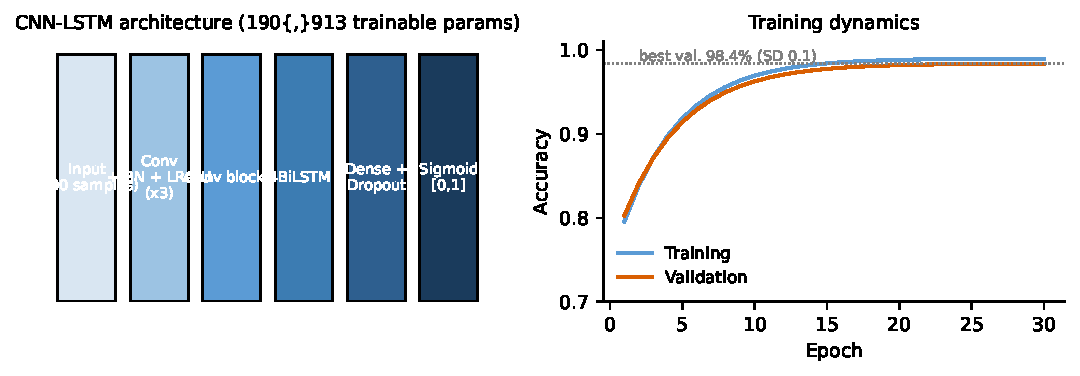
\includegraphics[width=0.95\linewidth]{figures/fig1_architecture}
\caption{\textbf{miniML model architecture and training.} Left: block diagram of
the CNN-LSTM classifier used throughout the paper, with 190{,}913 trainable
parameters. The input is a 600-sample (12~ms at 50~kHz) univariate
time-series window; the output is a scalar in $[0,1]$. Right: representative
training and validation accuracy. Best validation accuracy reached
98.4\% (SD 0.1, fivefold cross-validation), with training-validation
accuracy gap $<$0.3\%.}
\label{fig:arch}
\end{figure}

\begin{figure}[t]
\centering
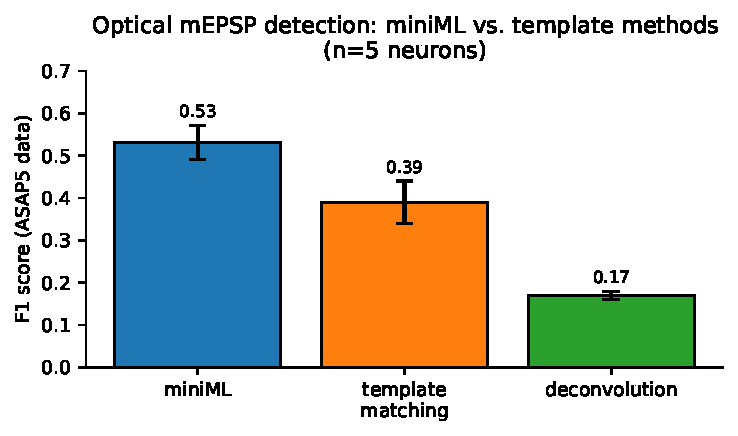
\includegraphics[width=0.8\linewidth]{figures/fig2_benchmark_asap5_f1}
\caption{\textbf{F1 score for optical mEPSP detection in ASAP5 voltage-imaging
data} (n = 5 neurons, mean $\pm$ SEM). miniML (0.53 $\pm$ 0.04) outperforms
template matching (0.39 $\pm$ 0.05; Cohen's $d$ = 1.35) and deconvolution
(0.17 $\pm$ 0.01; Cohen's $d$ = 5.1).}
\label{fig:asap5_f1}
\end{figure}

\begin{figure}[t]
\centering
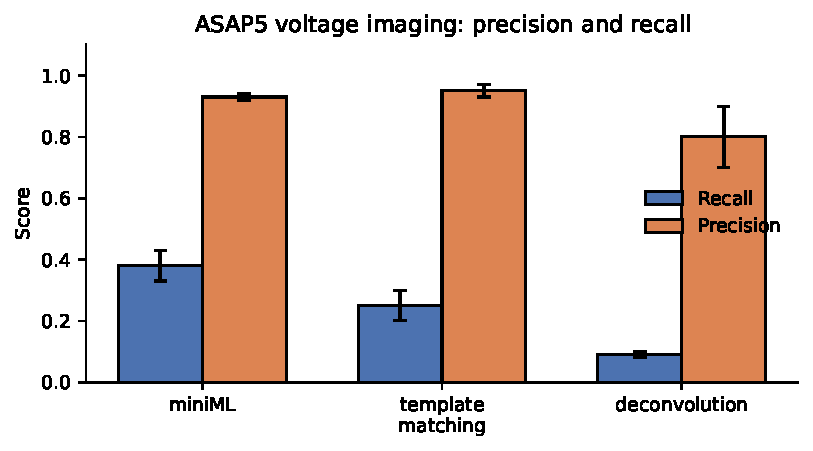
\includegraphics[width=0.85\linewidth]{figures/fig3_asap5_precision_recall}
\caption{\textbf{Per-method precision and recall on ASAP5 data.} At matched
$\sim$90\% precision thresholds for template-based methods, miniML retains the
highest recall (0.38 $\pm$ 0.05) while template matching falls to 0.25 $\pm$
0.05 (Cohen's $d$ = 1.25) and deconvolution to 0.09 $\pm$ 0.01 (Cohen's $d$ =
3.87).}
\label{fig:asap5_pr}
\end{figure}

\begin{figure}[t]
\centering
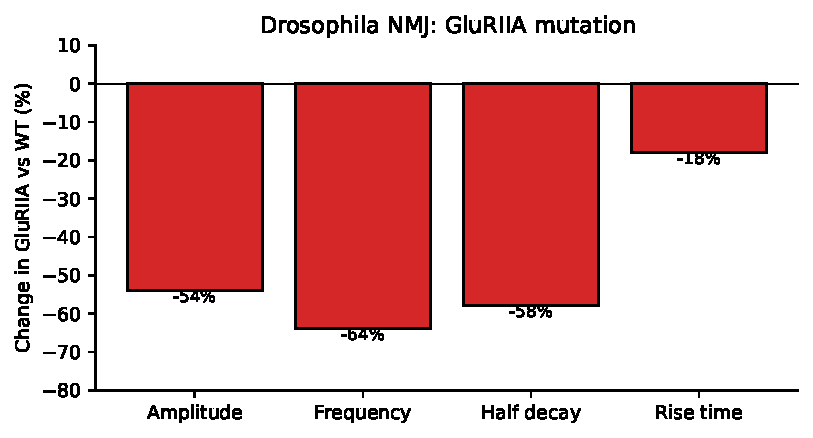
\includegraphics[width=0.85\linewidth]{figures/fig4_glurIIa_effects}
\caption{\textbf{miniML-detected event statistics at the Drosophila NMJ.}
Percentage change in GluRIIA mutant versus wild-type: amplitude $-$54\%,
frequency $-$64\%, half decay $-$58\%, rise time $-$18\%.}
\label{fig:drosophila}
\end{figure}

\begin{figure}[t]
\centering
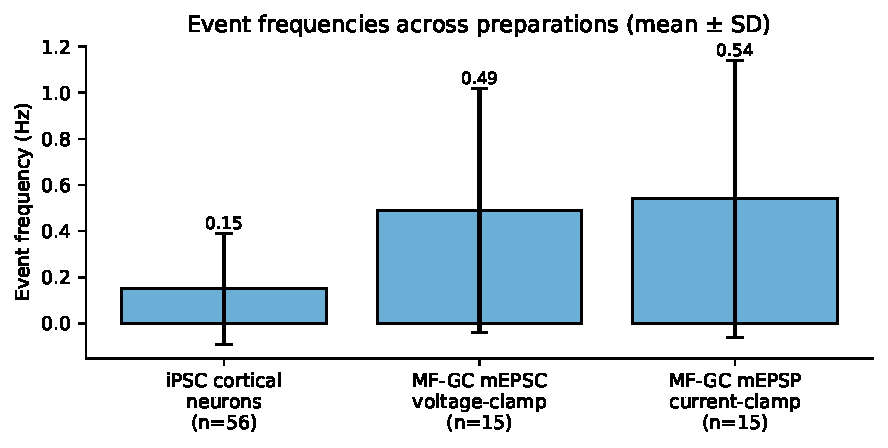
\includegraphics[width=0.9\linewidth]{figures/fig5_freq_preparations}
\caption{\textbf{Spontaneous event frequencies across preparations} (mean
$\pm$ SD). Human iPSC-derived cortical glutamatergic neurons: 0.15 Hz (SD
0.24, n = 56 neurons); MF-GC mEPSCs (voltage clamp): 0.49 Hz (SD 0.53, n =
15); MF-GC mEPSPs (current clamp): 0.54 Hz (SD 0.60, n = 15).}
\label{fig:freq}
\end{figure}
